\section{Project Development}
\subsection{Concept Development}
Over the next 10 years, the National Innovation Agency (NIA) has identified five major societal challenges related to mental health in Thailand. One of these challenges, dubbed “Terror Outbursts,” refers to incidents of violence or unrest fueled by unresolved societal issues. A deeper analysis reveals that stress and anxiety are significant concerns, with Thailand reporting an average stress rating of 7.7, highlighting the urgent need for intervention. While various solutions are available to address stress and anxiety, the team discovered that simply having someone to listen to is one of the most common and effective forms of support. However, there are moments when a person may not be available to offer comfort, which inspired the creation of Pookie.

Pookie draws inspiration from two key case studies: pets and desktop robots. Pets, such as dogs and cats, are often seen as a source of comfort and relaxation for their owners. Pookie’s design aims to emulate this same sense of comfort and relaxation through resemblance of a pet bear. On the other hand, emotional support robots combine sensors and software to interact with users. Pookie references these interactions and engineering, but adds on another key component that many robots lack: empathy.

With this in mind, the design of Pookie must adhere to two key pillars: empathy and interactivity. The user experience (UX) flow was carefully developed within this framework, which will be explored in the next section.

\subsection{User Experience Development}
\label{sec:ux}
To satisfy the key pillars of empathy and interactivity, the team initially developed the UX flow as shown in Figure \ref{fig:3-init}. According to the diagram, the user sets Pookie up in their home or working environment, and Pookie remains on throughout until the user turns it off. While on, Pookie analyzes the user’s facial and speech emotion, then provides an output personalized to each emotional status. This remained the as-is flowchart for the entirety of MVP 1 and half of MVP 2.

\begin{figure}[ht]
    \centering
    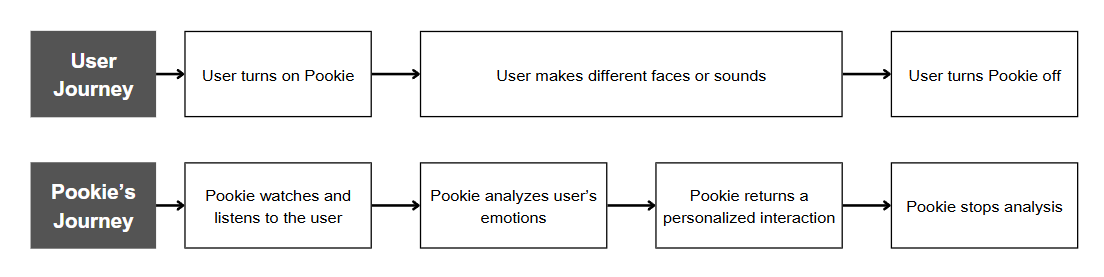
\includegraphics[width=\textwidth]{3-init.png}
    \caption{Initial UX Flowchart}
    \label{fig:3-init} 
\end{figure}

However, upon further empathizing with the user journey, this design lacked the interactivity element. To elaborate, simply having the robot stare at the user for a prolonged amount of time did not seem realistic, and turned out to be a very static design. To address this, the design had to be more dynamic and interactive. The team decided to add an activation layer to the user experience, allowing the user to activate Pookie’s functionalities and turn it off as they please. This was done through the use of \textbf{wake words}, a subset of voice recognition technologies aimed at identifying if a certain word was called out. This new flowchart is shown in Figure \ref{fig:4-revised}.

\begin{figure}[!ht]
    \centering
    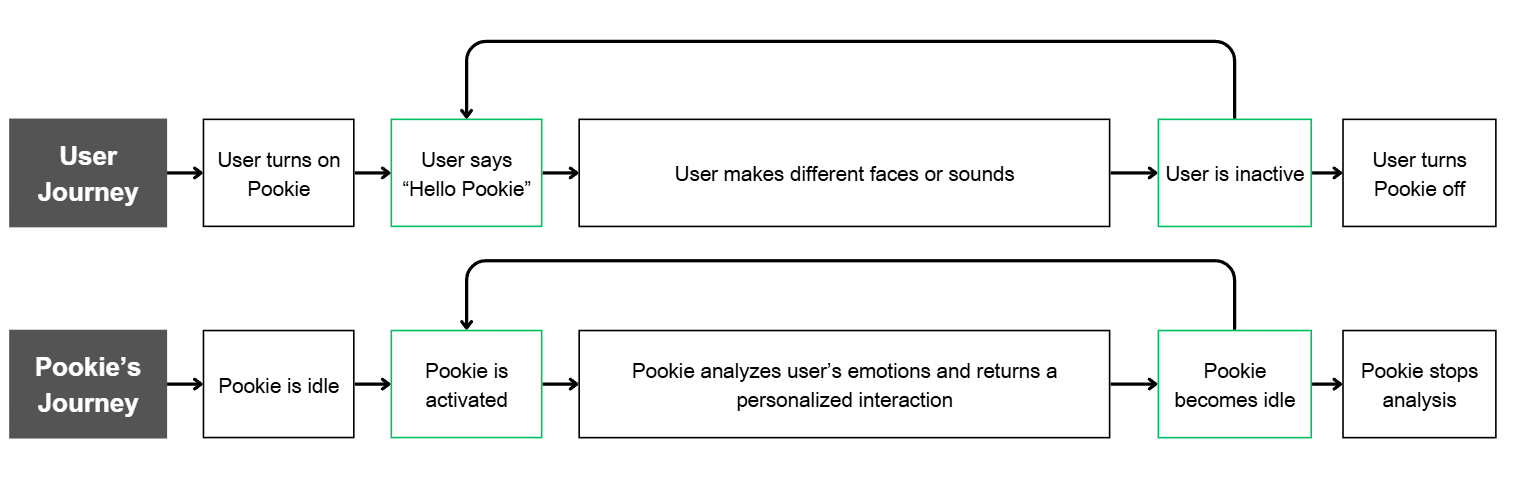
\includegraphics[width=\textwidth]{4-revised.png}
    \caption{Revised UX Flowchart}
    \label{fig:4-revised}
\end{figure}

To achieve this user experience, Pookie must have strong foundations in software and hardware design, being able to accurately determine the user’s emotions and seamlessly carrying out the physical interactions. The software and hardware development initiatives will be discussed in the next sections.

\subsection{Software Development}
In developing the software for Pookie, the tasks were split into 4 layers: activation, classification, decision, and output, as shown in Figure \ref{fig:5-software}. The activation layer represents the wake word “Hello Pookie” detection, which activates the real time input pipeline. Next, the classification layer processes data obtained from the camera and the microphone into the facial and speech emotion recognition models respectively. Moving forward, the decision layer consolidates the emotions detected from the classification layer into a single decision, which determines the output in the output layer. This section will discuss each layer in detail, discussing the rationales behind each technology, results, and challenges.

\begin{figure}[!ht]
    \centering
    \captionsetup{justification=centering}
    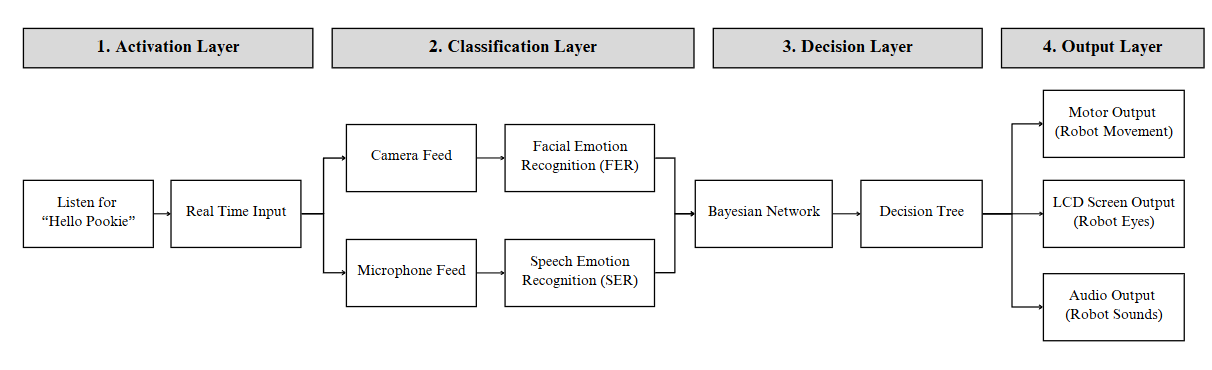
\includegraphics[width=\textwidth]{5-software.png}
    \caption{Software Flowchart}
    \label{fig:5-software}
\end{figure}

\subsubsection{Activation Layer}
The activation layer is primarily responsible for wake word detection—identifying a specific keyword that activates or essentially "wakes up" Pookie. However, developing a precise wake word model from scratch presents numerous challenges and can be a time-consuming process. Given that this was not the central focus of our project, we aimed for a more efficient solution.

Fortunately, Picovoice.ai offers a ready-to-use tool called Porcupine, which enables users to simply input a keyword and generate an offline-compatible model \cite{picovoice_porcupine}. Our team adopted this technology as a rapid and effective addition to the system.

The only challenge we encountered was that Pookie's software was designed to run on the Jetson Orin, which uses an aarch64 architecture and ARM CPU. This caused compatibility issues with some dependencies, especially the Pyporcupine wake word detection library, which is typically tailored for specific hardware platforms. To solve this, we spoofed the Jetson Orin Nano as a Raspberry Pi 5, as both devices run on the same ARM CPU architecture and use the aarch64 instruction set. This allowed us to bypass platform-specific constraints and successfully run Pyporcupine on the Orin.

\subsubsection{Classification Layer}
\label{sec:classification-layer}
The classification layer comprises two essential AI models: the facial and speech emotion recognition models. On one hand, the facial emotion recognition model leverages convolutional neural network (CNN) technologies to learn and extract features from a dataset of faces. On the other hand, the speech emotion recognition model leverages bidirectional long short term memory (LSTMs) to classify speech into respective emotions. It is important to note that the FER model classifies emotions under the seven universal emotions criteria, but the speech emotion recognition model is trained to classify only five. 

In terms of facial emotion recognition, two components must be obtained: the dataset and the model. Regarding the dataset, the facial expression recognition model was trained on a Chinese Faces Dataset , chosen for its similar characteristics to the hard-to-obtain Thai dataset. Utilizing an intuitive approach to synthetic data generation, the dataset was based on a Chinese Face Dataset with Dynamic Expressions and Diverse Ages Synthesized by Deep Learning \cite{han2023}, where a team of researchers created a facial expression image generation model for various Chinese faces belonging to different age groups, genders, and face structure, as shown in Figure \ref{fig:6-face}, labeled as “Ours”. 

\begin{figure}[!ht]
    \centering
    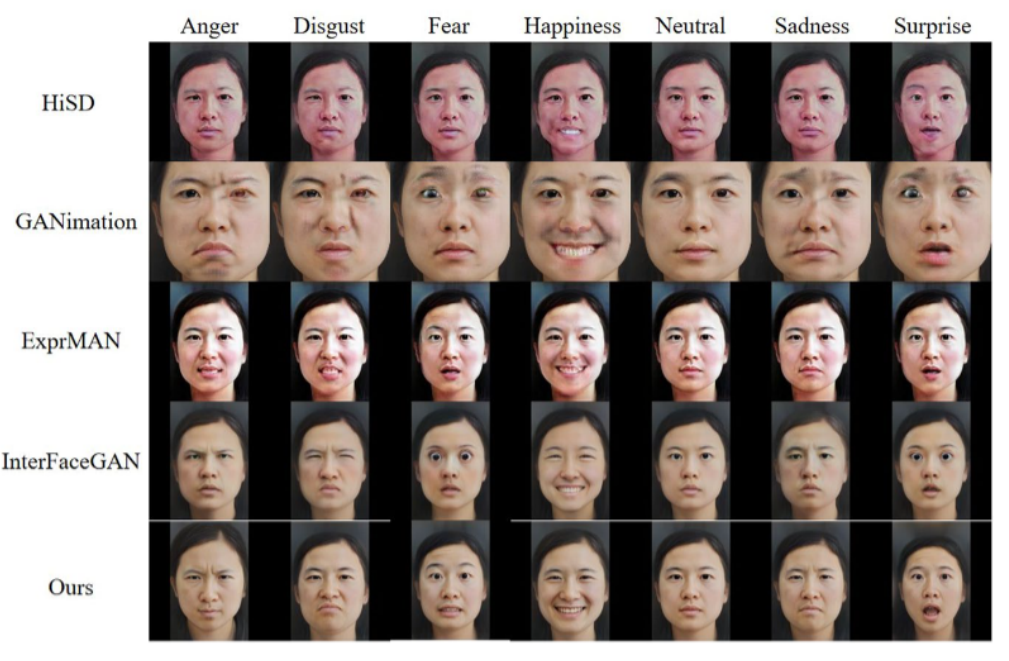
\includegraphics[width=0.8\textwidth]{6-face.png}
    \captionsetup{justification=centering}
    \caption{A Chinese Face Dataset with Dynamic Expressions and Diverse Ages Synthesized. Source: Adapted from \cite{han2023}}
    \label{fig:6-face}
\end{figure}

In terms of model selection, the team utilized three criteria for evaluation: speed, size, and training complexity. Firstly, the model must be fast enough to perform inferences on a real time video feed with minimal latency. Secondly, the size of the model must be lightweight, and highly compatible with the Jetson Orin. Lastly, it must not be too complex to train, with little to no need for additional hyperparameter tuning. 

Upon further analysis, the team singled down on using the VGGNet architecture (Figure \ref{fig:7-vggnet}) —a multi-layer convolutional neural network renowned for feature extraction and classification, particularly in emotion detection models \cite{simonyan2015deepconvolutionalnetworkslargescale}. The decision to select VGGNet was influenced by its balance between performance and implementation simplicity. Although newer architectures like ResNet or EfficientNet offer improved accuracy and deeper representations, they tend to demand more computational resources and training time, which would compromise the low-latency requirement of the system. VGGNet, on the other hand, provides a straightforward layer structure that is easier to deploy on edge devices such as the Jetson Orin, especially when pre-trained weights are utilized.

\begin{figure}[!ht]
    \centering
    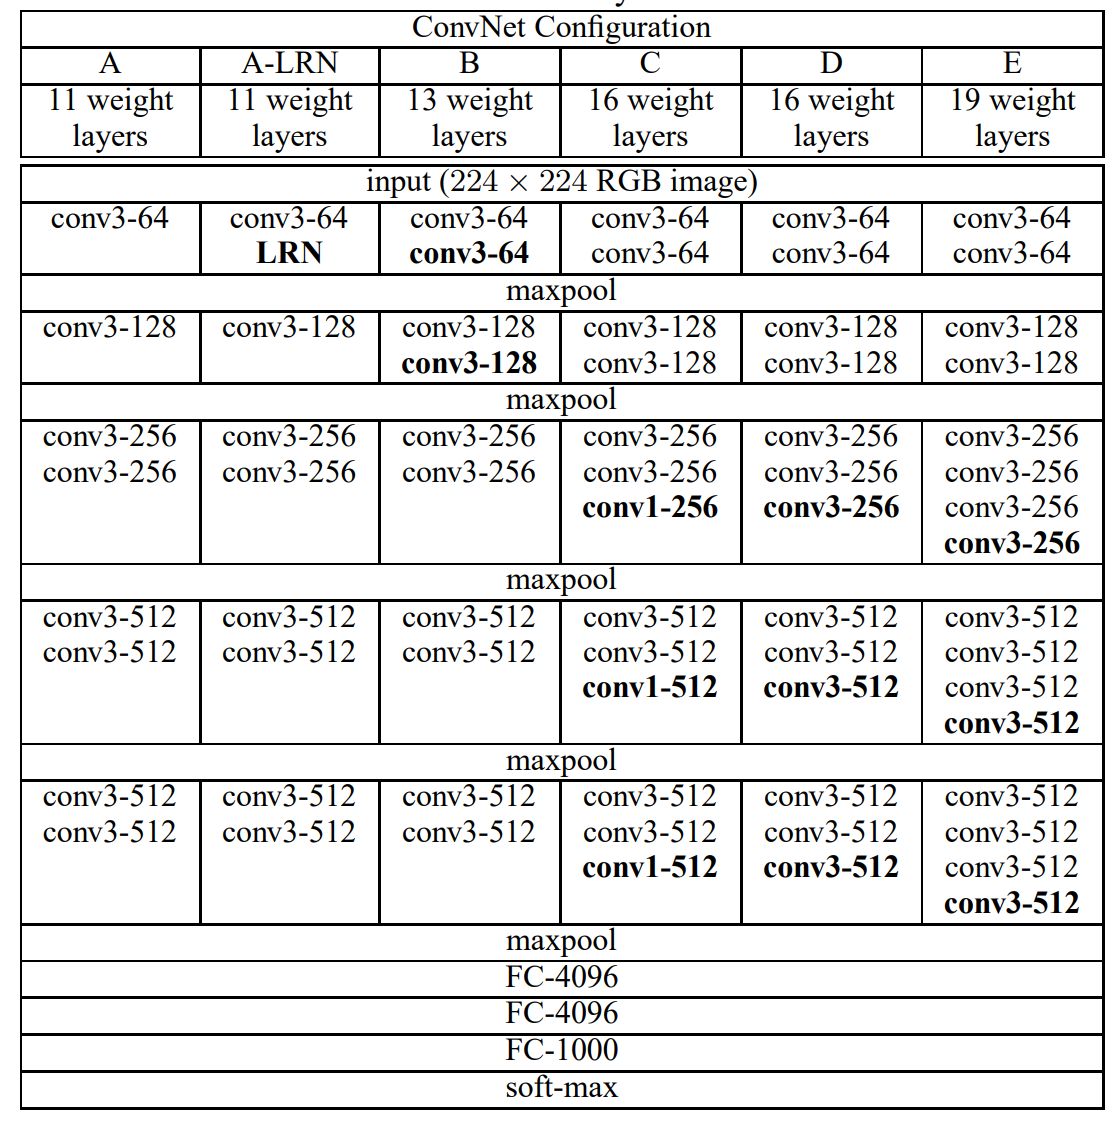
\includegraphics[width=0.75\textwidth]{7-vggnet.png}
    \captionsetup{justification=centering}
    \caption{VGGNet Architecture. Source: Adapted from \cite{simonyan2015deepconvolutionalnetworkslargescale}}
    \label{fig:7-vggnet}
\end{figure}

Thus, the team trained the VGGNet architecture from scratch using the dataset of Chinese faces discussed earlier. Overall, the training results were better than expected, as shown in Table \ref{tab:8-test}, where the model is great at distinguishing between positive emotions such as happiness or surprise, but it is quite lacking in negative emotions. However, given the scope of the project, where positive and neutral are associated with specific outputs, and negative emotions are generally classified as stress, then the model is generally enough to use as a minimum viable product.

\begin{table} [!ht]
    \centering
    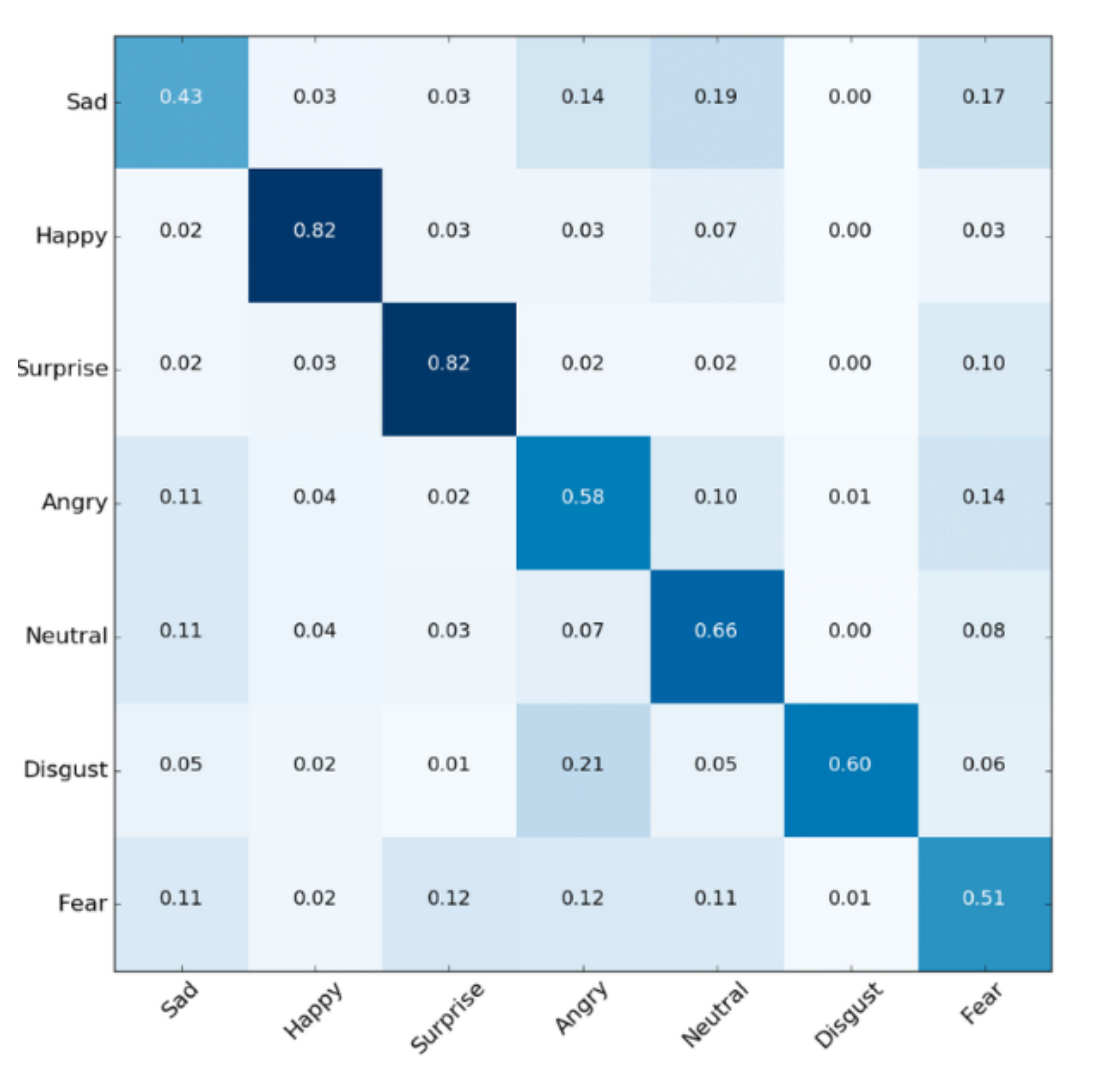
\includegraphics[width=0.7\textwidth]{8-test.png}
    \captionsetup{justification=centering}
    \caption{VGGNet Model Evaluation (Testing Set)}
    \label{tab:8-test}
\end{table}

\newpage
On the other hand, in terms of the speech emotion recognition dataset, the team leveraged a recently published open source Thai Speech Emotion Dataset from VISTEC-depa Thailand AI Research Institute \cite{vistec_ai_ser}, which provides an open source dataset of studio recorded voices with five labels: neutral, anger, happiness, sadness, frustration. The dataset comprises 41 hours and 27,854 sentences of studio recorded voices, with over 200 studio actors. To train this model, VISTEC-depa also utilized a Convolutional Neural Network-Bidirectional Long Short-Term Memory (CNN-BiLSTM) architecture, as shown in Figure \ref{fig:9-lstm}. speech for emotion classification through four stages: converting audio to mel-scale spectrograms, extracting features with 1D CNN and LeakyReLU, capturing temporal patterns via Bidirectional LSTM, and classifying emotions through a Softmax layer. Trained on the VISTEC-depa Thai Speech Emotion Dataset (41 hours, 27,854 sentences from 200+ actors), this hybrid model effectively recognizes five emotions (neutral, anger, happiness, sadness, frustration) by combining CNN's spatial feature extraction with BiLSTM's sequential processing capabilities.

\begin{figure} [!ht]
    \centering
    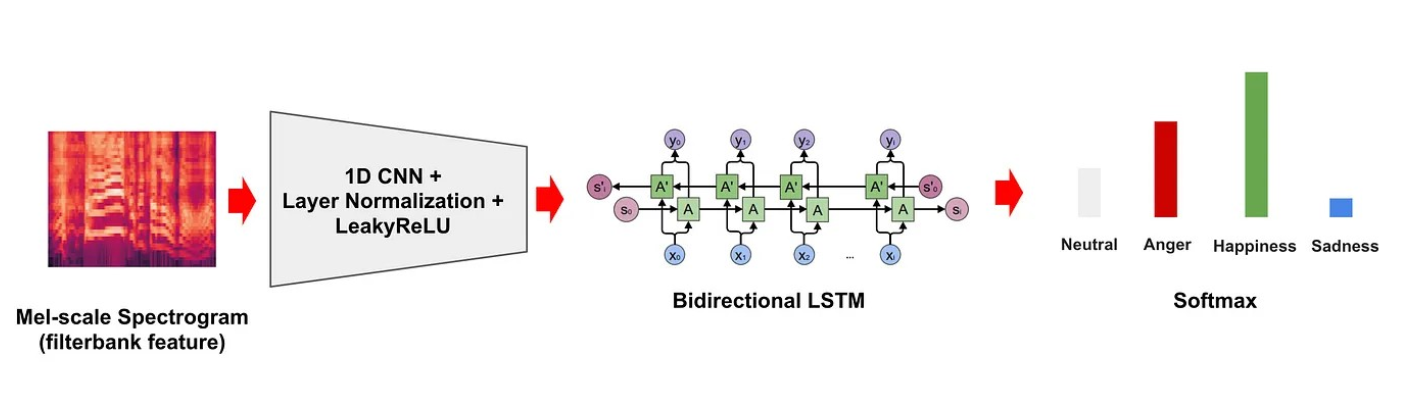
\includegraphics[width=\textwidth]{9-lstm.png}
    \captionsetup{justification=centering}
    \caption{CNN-LSTM Architecture. Source: Adapted from \cite{vistec_ai_ser}}
    \label{fig:9-lstm}
\end{figure}

In terms of evaluation, the CNN-BiLSTM model demonstrated solid performance across all emotional categories, with particularly strong accuracy in identifying neutral speech patterns. Notably, this represents one of the few publicly available Thai speech emotion recognition systems in existence. Given these strengths, the development team integrated this architecture into Pookie for real-time emotion inference capabilities, enabling dynamic emotional assessment during live interactions.

\begin{table} [!ht]
    \centering
    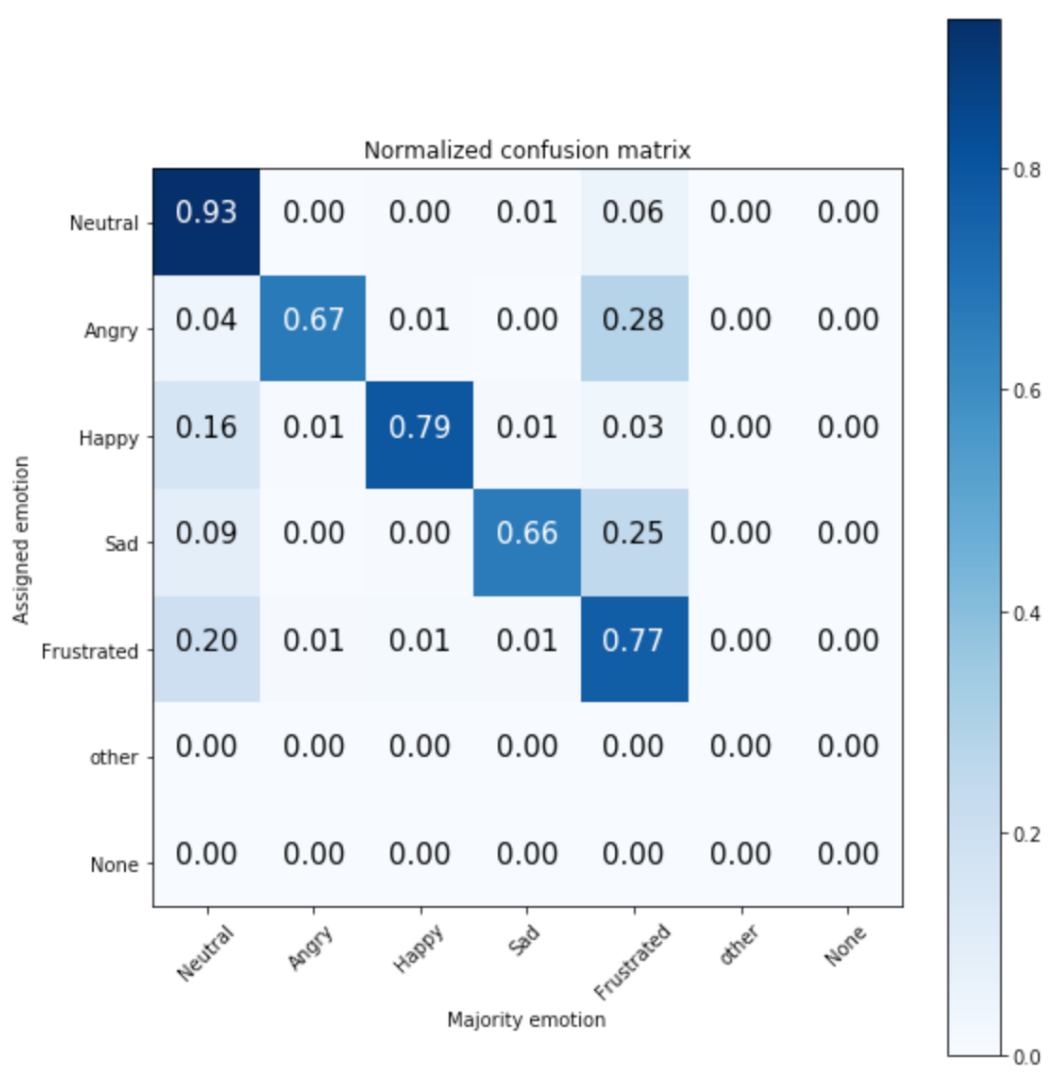
\includegraphics[width=0.7\textwidth]{10-ser.png}
    \captionsetup{justification=centering}
    \caption{SER Model Evaluation. Source: Adapted from \cite{vistec_ai_ser}}
    \label{tab:10-ser}
\end{table}

\subsubsection{Decision Layer}
While Pookie can now successfully determine the user’s emotion through their face and speech, it does not answer the main question: what is the user actually feeling? This cannot be answered easily, as the models produce different sets of outputs, leading to potential ambiguity. For context, each of the FER and SER emotions output a JSON of probabilities and their confidence (e.g Happiness 60\%, Neutral 30\%, Anger 10\%), with the potential outputs from each model shown in Table \ref{tab:11-mapping}. As shown in the figure, the models do not produce outputs with a 1:1 relationship, meaning some emotions from FER do not have a SER counterpart (such as FER output “Fear” does not have a corresponding emotion on the SER side).

\begin{table}[h]
    \centering
    \begin{tabular}{|c|c|}
        \hline
        \textbf{Facial Emotion Recognition (FER) Outputs} & \textbf{Speech Emotion Recognition (SER) Outputs} \\
        \hline
        Neutral   & Neutral   \\
        \hline
        Anger     & Anger     \\
        \hline
        Happiness & Happiness \\
        \hline
        Sadness   & Sadness   \\
        \hline
        Disgust   & Frustration \\
        \hline
        Fear      & Sadness (SER)   \\
        \hline
        Surprise  & Neutral (SER)   \\
        \hline
    \end{tabular}
    \caption{Mapping of Emotions for SER and FER}
    \label{tab:11-mapping}
\end{table}

To address this ambiguity, the use of Bayesian networks and decision trees were introduced within the pipeline. The purpose was to consolidate the distributions of emotion recognition confidence from the two models into one source of truth: what the user is theoretically feeling. 

A Bayesian Network is a probabilistic graphical model that represents a set of variables and their conditional dependencies using a directed acyclic graph (DAG). It provides a structured approach to reasoning under uncertainty by encoding the probabilistic relationships between variables. In the context of Pookie, the Bayesian Network is used to infer the user’s true emotional state by integrating evidence from both the FER and SER models. The revised implementation introduces a Bayesian Network shown in Figure \ref{fig:12-bayes}, where the user’s underlying emotional state is treated as a latent variable, which is updated dynamically as new observations from FER and SER arrive. The network consists of nodes representing possible emotions and edges that define the probabilistic dependencies between them. Given an initial prior belief about the user’s emotion, the system updates its belief by incorporating new observations from the FER and SER models using Bayes’ Theorem.

\begin{figure}[!ht]
    \centering
    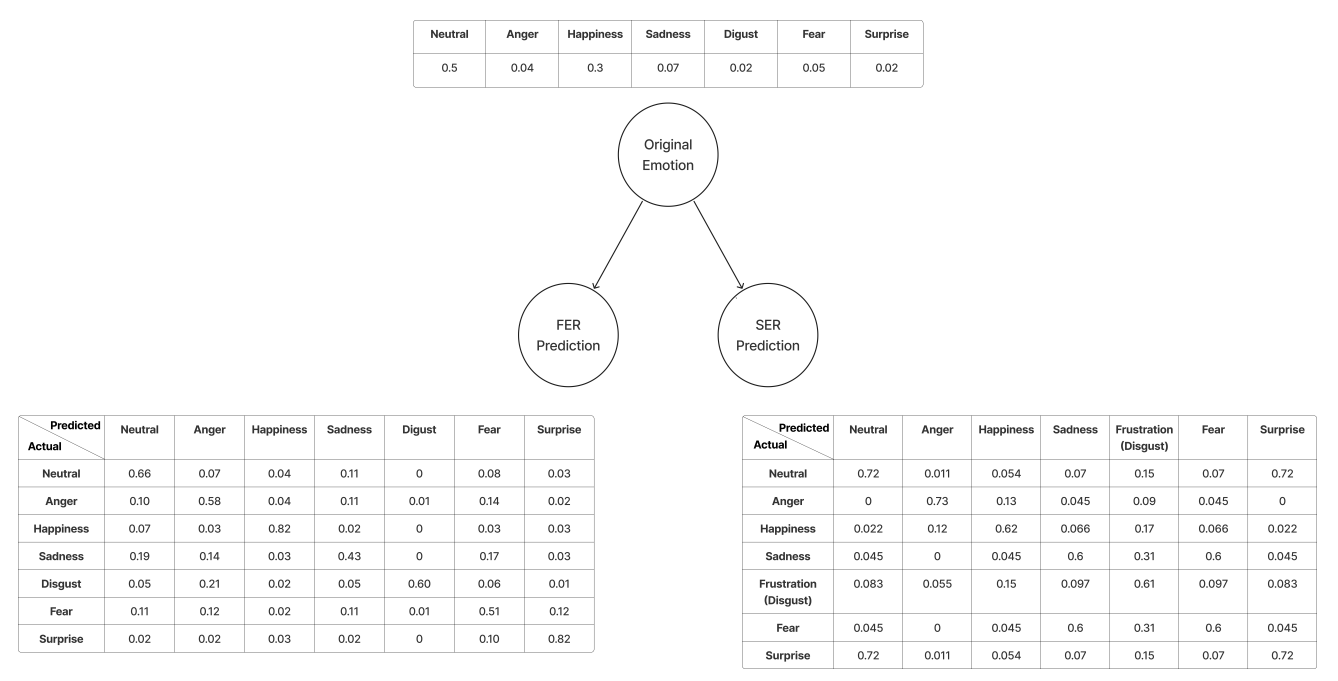
\includegraphics[width=\textwidth]{12-bayes.png}
    \captionsetup{justification=centering}
    \caption{Pookie’s Bayesian Network}
    \label{fig:12-bayes}
\end{figure}

To construct the Bayesian Network, we defined conditional probability tables (CPTs) based on confusion matrices from both the FER and SER models seen in Tables \ref{tab:8-test} and \ref{tab:10-ser} respectively, as well as insights from Emotions in Everyday Life by Trampe et al. (2015) \cite{10.1371/journal.pone.0145450}, which provides probability distributions of emotions. By analyzing the confusion matrices, we estimated the likelihood of misclassifications and incorporated these probabilities into the CPTs, ensuring a more accurate representation of emotional relationships. 

The confusion matrices represent how often the models correctly and incorrectly classify different emotional states. By utilizing these matrices, we were able to estimate the conditional probabilities for each emotional state. For example, if the FER model often misclassifies "Fear" as "Surprise" or "Sadness," these relationships are reflected in the CPTs. Similarly, if the SER model has a tendency to confuse "Frustration" with "Anger," the Bayesian Network accounts for these uncertainties when updating its belief about the user’s true emotion.

By combining the confusion matrix data with the probability distributions from the research paper, we constructed CPTs that better capture real-world emotional correlations. This approach allows the Bayesian Network to weigh the reliability of each model's predictions and adjust the estimated emotional state accordingly. Instead of treating FER and SER outputs as absolute truths, the system considers their likelihood of being correct based on historical performance.

To update the belief about the user’s emotional state, the Bayesian Network relies on Bayes’ Theorem, which provides a framework for calculating conditional probabilities. Specifically, the network uses the formula:

\begin{gather}
    P(E \mid R) = \frac{P(R \mid E) \cdot P(E)}{P(R)}
\end{gather}

Where:
\begin{itemize}
    \item \( P(E \mid R) \) is the posterior probability, representing the probability of the emotional state \( E \) given the result \( R \) (i.e., the FER and SER outputs).
    \item \( P(R \mid E) \) is the likelihood, which indicates how likely the result \( R \) is, given the emotional state \( E \).
    \item \( P(E) \) is the prior probability, representing the initial belief about the emotional state before observing the result, which is informed by the emotion distribution provided in \textit{Emotions in Everyday Life} by Trampe et al. (2015) \cite{10.1371/journal.pone.0145450}.
    \item \( P(R) \) is the evidence, or the total probability of observing the result under all possible emotional states.
\end{itemize}

In the context of Pookie, the emotional state \( E \) could be one of the possible emotions such as happiness, sadness, anger, etc. The result \( R \) is derived from the outputs of the FER and SER models, which provide a set of probabilities for each emotion. The likelihood \( P(R \mid E) \) is determined by the confusion matrices of the FER and SER models, which reflect how likely it is for the models to generate certain outputs given the true emotional state.

In this case, the likelihood \( P(R \mid E) \) is represented as the product of the probabilities from both the Facial Emotion Recognition (FER) and Speech Emotion Recognition (SER) models. Since we are dealing with two different models that provide independent estimates of the user’s emotional state, we combine these estimates by multiplying their corresponding probabilities for each emotion.

Thus, the likelihood for each possible emotional state \( E \) given the result \( R \) (which consists of the outputs from both the FER and SER models) can be expressed as:

\begin{gather}
    P(R \mid E) = P(R_{\text{FER}} \mid E) \cdot P(R_{\text{SER}} \mid E)
\end{gather}


Where:
\begin{itemize}
    \item \( P(R_{\text{FER}} \mid E) \) is the probability of the FER result \( R_{\text{FER}} \) given the emotional state \( E \).
    \item \( P(R_{\text{SER}} \mid E) \) is the probability of the SER result \( R_{\text{SER}} \) given the emotional state \( E \).
\end{itemize}

Since the FER and SER models are independent, their combined likelihood is simply the product of their individual likelihoods. This approach assumes that facial and speech expressions are conditionally independent given the true emotional state. By multiplying the probabilities, we take into account both the visual and auditory evidence of the user’s emotion, and use the combined evidence to estimate the true emotional state more accurately.

Thus, the updated Bayesian formula for computing the posterior probability of the emotional state \( E \) given the observations \( R_{\text{FER}} \) and \( R_{\text{SER}} \) becomes:

\begin{gather}
    P(E \mid R_{\text{FER}}, R_{\text{SER}}) = \frac{P(R_{\text{FER}} \mid E) \cdot P(R_{\text{SER}} \mid E) \cdot P(E)}{P(R_{\text{FER}}, R_{\text{SER}})}
\end{gather}

Where:
\begin{itemize}
    \item \( P(R_{\text{FER}}, R_{\text{SER}}) \) is the evidence or the total probability of observing both the FER and SER results. This is computed as the sum of the likelihoods over all possible emotional states:
\end{itemize}

\begin{gather}
    P(R_{\text{FER}}, R_{\text{SER}}) = \sum_{E} P(R_{\text{FER}} \mid E) \cdot P(R_{\text{SER}} \mid E) \cdot P(E)
\end{gather}

This formulation ensures that the system updates its belief about the user's emotional state by considering the likelihood of both the FER and SER outputs for each possible emotion. By combining the results from the facial and speech emotion recognition models, the Bayesian Network effectively integrates multiple sources of evidence, resulting in a more robust and accurate estimate of the user's true emotional state.

The use of multiplication for the likelihoods allows the Bayesian Network to properly account for the evidence from both modalities, reducing the impact of uncertainties and ambiguities from individual models. This approach improves the overall accuracy of the emotional assessment and enhances the robot's ability to make decisions that align with the user's true feelings.

The prior \( P(E) \) is based on a generalized distribution of emotional states, derived from external research, such as the findings from \cite{10.1371/journal.pone.0145450}. It reflects the average emotional distribution across a population and does not adjust based on an individual user’s history or context. This prior probability serves as a baseline, representing the general likelihood of each emotional state before any new observations from the FER and SER models are made.

Finally, \( P(R) \), the evidence, ensures that the posterior probabilities of all possible emotional states sum to 1. This value can be calculated as the sum of the likelihoods over all possible emotional states:

\begin{gather}
    P(R) = \sum_{E} P(R \mid E) \cdot P(E)
\end{gather}

By applying Bayes’ Theorem iteratively as new observations from the FER and SER models arrive, the Bayesian Network updates its belief about the user's emotional state. This update does not involve refining the estimate based on previous emotional history, but rather adjusts the system’s estimate by integrating the evidence from the two models in real time. This process allows the system to more accurately infer the user’s emotional state and navigate complex emotional situations with greater precision, reducing ambiguity and improving the overall user experience.

This probabilistic model enables Pookie to move beyond simple rule-based decision-making and handle the complexity of real-world emotional states more effectively.

The calculated outputs from the Bayesian network are passed onto a custom decision tree, comprising various nodes containing conditions and actions. The decision tree references the framework shown in Figure \ref{fig:2-framework} to determine the type of action, where the Bayesian network and other data processing pipelines produces an output that is classified into positive, neutral, or negative. With each type of emotion, Pookie then decides whether or not to maintain, enhance, or empathize with the emotion. 

\begin{figure}[ht]
    \centering
    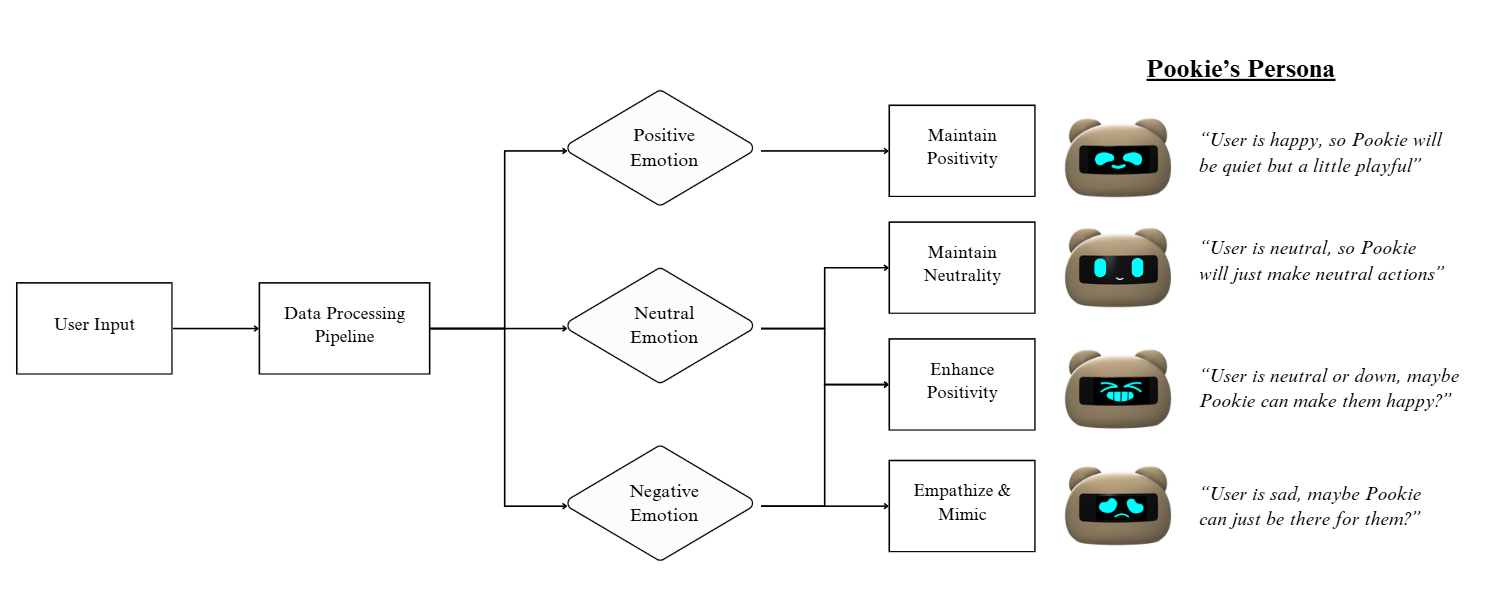
\includegraphics[width=\textwidth]{2-flow.png}
    \captionsetup{justification=centering}
    \caption{Framework for Action Classification}
    \label{fig:2-framework}
\end{figure}

The decision tree consists of 7 branches and a total of 65 nodes with each branch representing a specific dominant emotion. Subsequent layers correspond to conditional checks that help determine the most appropriate action for Pookie to take. An example of such a branch is illustrated in Figure \ref{fig:13-dt}. As shown in the diagram, the initial layer evaluates the output from the Bayesian network to assess whether the dominant emotion is neutral. The following layers then apply additional filters—such as verifying whether positive emotions outweigh negative ones—to further refine the decision. Ultimately, an action is selected based on the emotional state. For example, if the user exhibits predominantly negative emotions, Pookie may respond by making playful eye gestures to uplift the user's mood, an action categorized as “positive enhancement.”

\begin{figure}[ht]
    \centering
    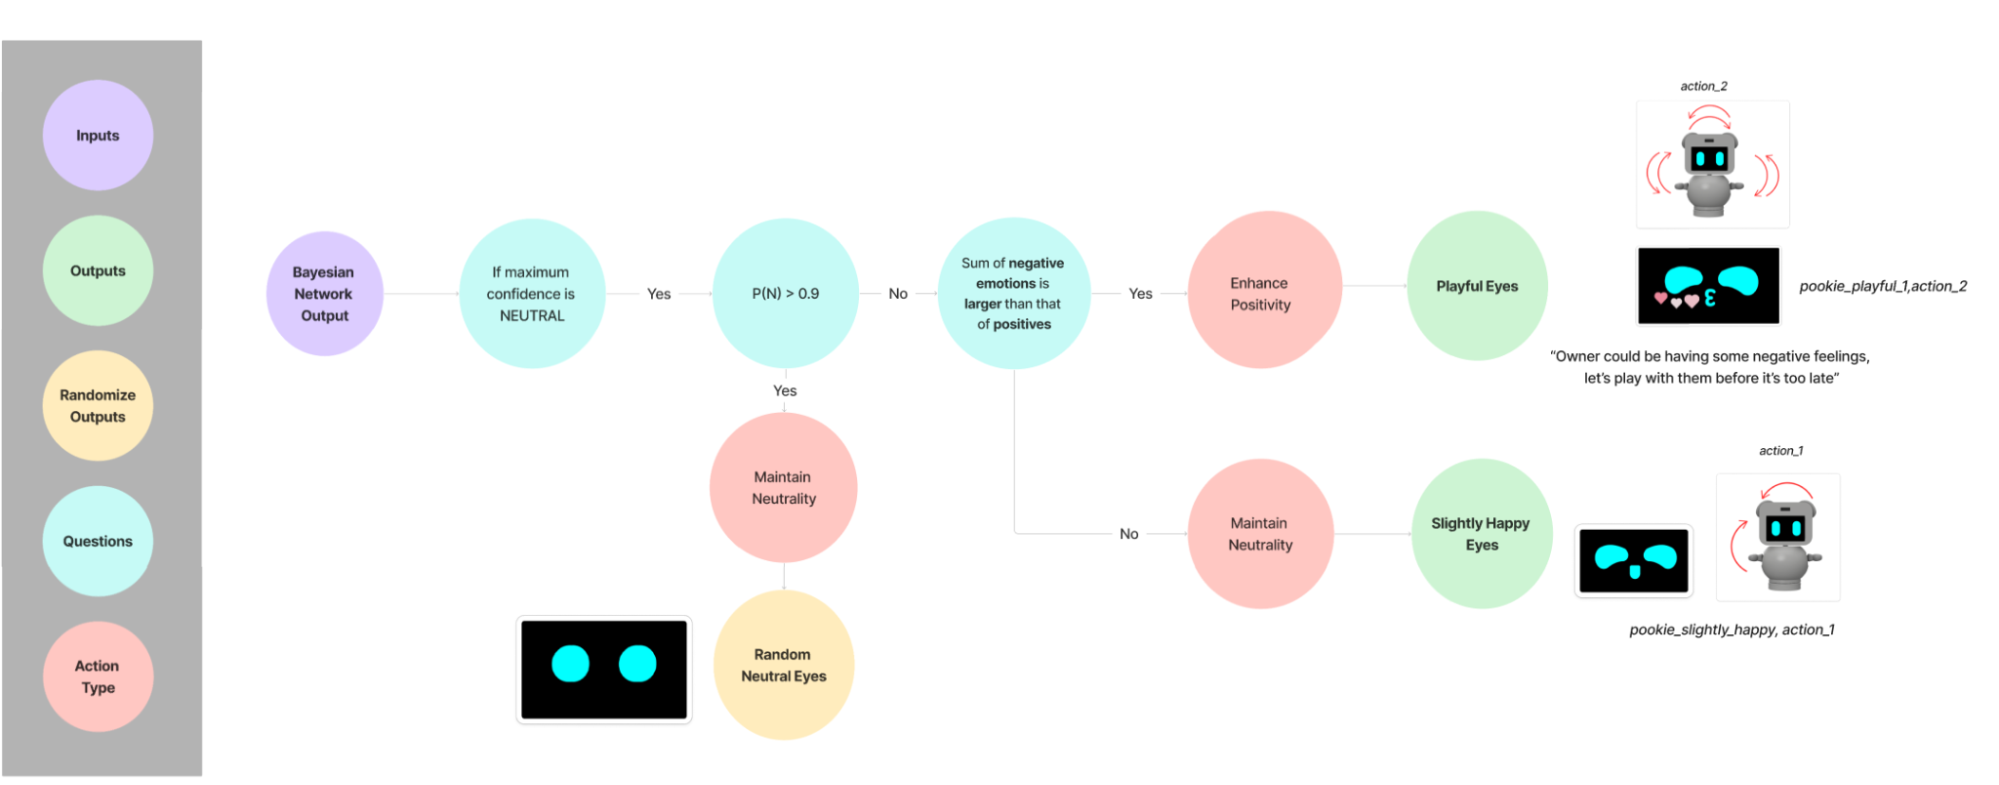
\includegraphics[width=\textwidth]{13-dt.png}
    \captionsetup{justification=centering}
    \caption{Decision Tree Example}
    \label{fig:13-dt}
\end{figure}

\subsubsection{Output Layer}
Finally, the output layer comprises three actions: eye movement, physical movement, and sound. Firstly, the eye patterns are delivered through the LCD Screen as a sequence of frames in a Graphics Interchange Format (GIF). Some examples of eye representations are shown in Figure \ref{fig:14-eye}. These sequences of eye frames were created in Canva, a web application for making powerpoint slides or sequences of images, where the team has built a total of 20 different eye frames to give Pookie another level of interaction.

\begin{figure}[!ht]
    \centering
    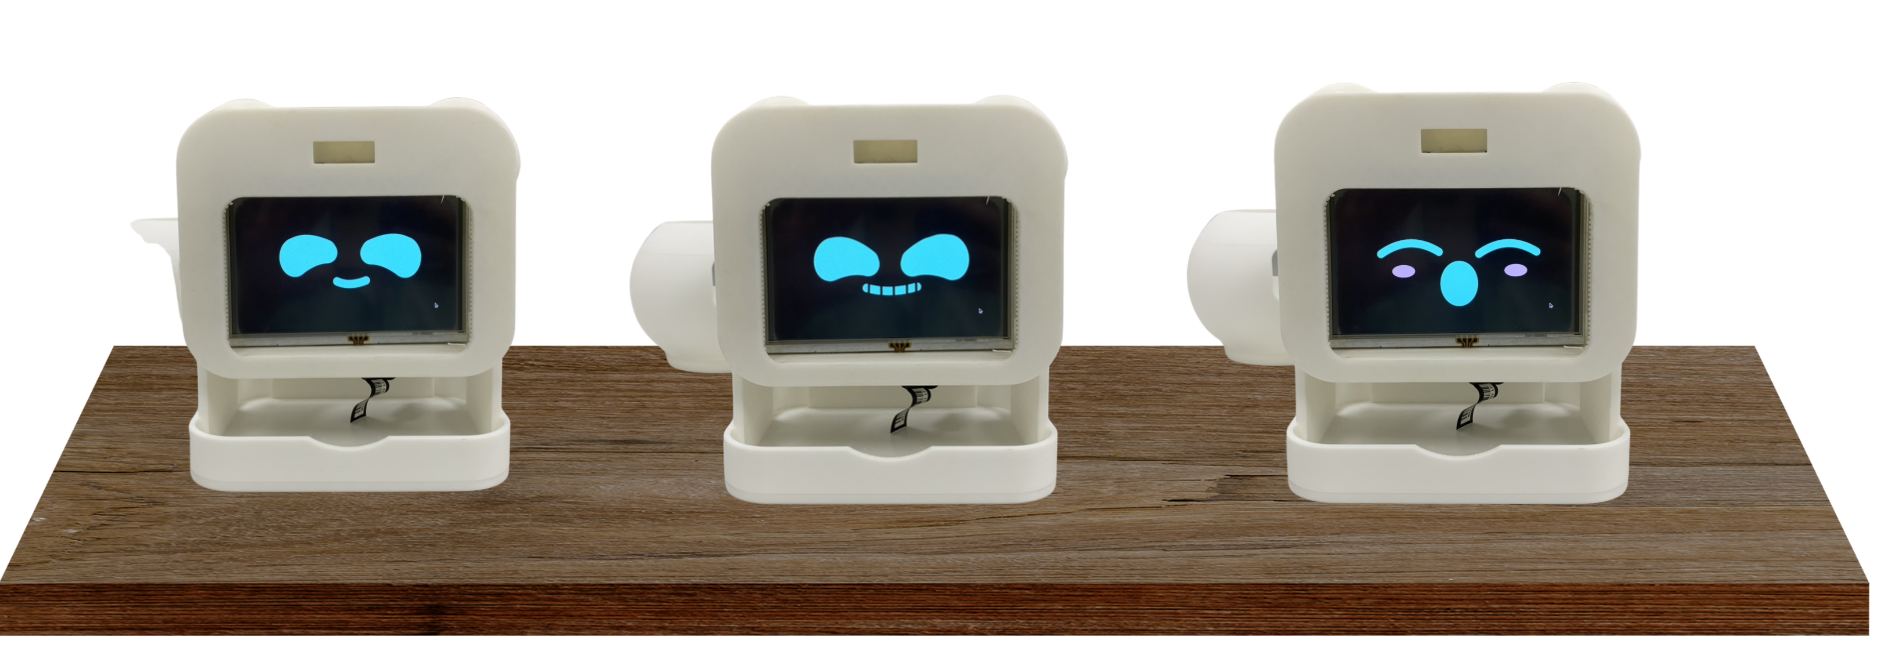
\includegraphics[width=\textwidth]{14-eye.png}
    \captionsetup{justification=centering}
    \caption{Pookie Eye Examples}
    \label{fig:14-eye}
\end{figure}

\newpage
Next, the physical movement patterns were manually programmed to align with the decision tree and framework described in the previous section. Figure \ref{fig:15-move} showcases examples of the movements Pookie is capable of performing. Specifically, Pookie possesses four axes of motion—located at its neck, two arms, and base—which enable it to engage in expressive, interactive behavior with the user.

\begin{figure}[!ht]
    \centering
    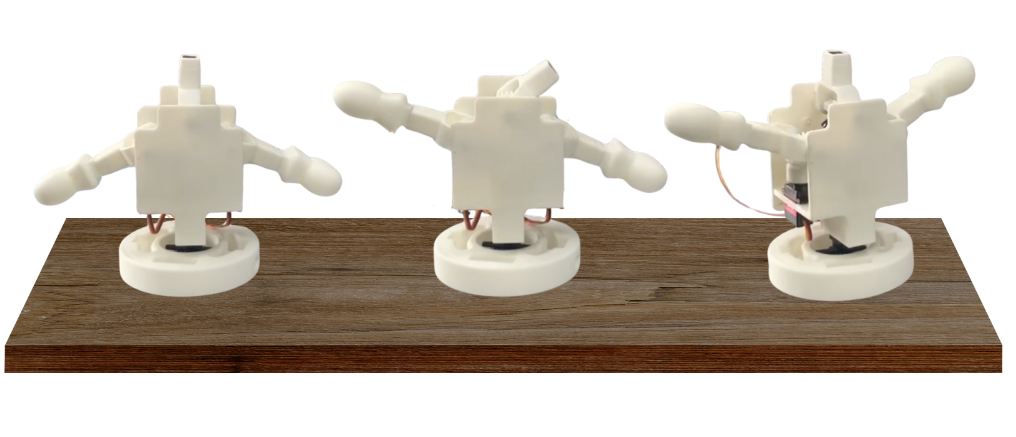
\includegraphics[width=\textwidth]{15-move.png}
    \captionsetup{justification=centering}
    \caption{Pookie Body Movements (Interior)}
    \label{fig:15-move}
\end{figure}

Lastly, sound effects were integrated using an open-source platform called Epidemic Sound, which offers a wide range of royalty-free sound effects for download. These audio elements were selected to complement Pookie’s actions and enhance user interaction.

\subsection{Software Pipeline Evaluation}

\subsubsection{Experiment Overview}
For each output theme, 10 trials were conducted to evaluate the consistency of the emotion pipeline. In each trial, the tester assumed an emotion, after which \textit{Pookie} predicted the emotion and generated a corresponding output. If the assumed emotion and the predicted emotion matched, the trial was labeled as an \textbf{\textit{Intended Result}}.

\newpage
\subsubsection{Remarks}
\begin{itemize}
    \item Results caused by identifiable bugs were excluded. Potential bugs included:
    \begin{itemize}
        \item The robot unexpectedly transitioning to a sleep state.
        \item Asynchronous behavior in the robot's outputs.
    \end{itemize}
    \item The experiment may contain inherent bias:
    \begin{itemize}
        \item Testers were deliberately expressing specific emotions, which does not fully reflect real-world circumstances.
    \end{itemize}
    \item Based on statistical calculations, a total of 246 trials would be required to achieve a 95\% confidence level in the overall evaluation.
\end{itemize}

\subsubsection{Confidence Level Calculation}
To determine the number of trials required for evaluating the emotion pipeline with statistical confidence, we used the following standard formula for estimating sample size in proportion-based accuracy testing:

\[
n = \left(\frac{Z^2 \cdot p\cdot(1 - p)}{E^2}\right)
\]

Where:
\begin{itemize}
    \item \( n \) is the required sample size,
    \item \( Z \) is the z-score corresponding to the desired confidence level,
    \item \( p \) is the estimated accuracy (proportion of intended results),
    \item \( E \) is the acceptable margin of error.
\end{itemize}

For a 95\% confidence level, we use \( Z = 1.96 \). Assuming an estimated accuracy of \( p = 0.80 \), and a margin of error \( E = 0.05 \), the calculation is:

\[
n = \left(\frac{1.96^2 \cdot 0.8 \cdot (1 - 0.8)}{0.05^2}\right)
\approx 246
\]

Thus, approximately 246 trials are needed to evaluate the pipeline with a 95\% confidence level and a ±5\% margin of error.

\subsubsection{Results}
\begin{enumerate}
    \item \textbf{Emotional Maintenance:} \textit{90\%} of trials were successful.
    \begin{table}[!ht]
        \centering
        \resizebox{\textwidth}{!}{
        \begin{tabular}{|c|l|l|l|l|l|}
        \hline
        \textbf{Trials} & \textbf{Forms of Input} & \textbf{Prediction} & \textbf{Assumed Action} & \textbf{Actual Action} & \textbf{Remarks} \\
        \hline
        1 & FER Only (Slight Smile) & Happiness 62.4\% & Slightly Happy / Very Happy & Slightly Happy & Intended Result \\
        \hline
        2 & FER Only (Normal Smile) & Happiness 74.0\% & Slightly Happy / Very Happy & Very Happy & Intended Result \\
        \hline
        3 & FER Only (Exaggerated Smile) & Happiness 82.1\% & Slightly Happy / Very Happy & Slightly Happy & Intended Result \\
        \hline
        4 & FER Only (Surprised Face) & Surprise 64.6\% & Surprise 3 & Surprise 3 & Intended Result \\
        \hline
        5 & FER Only (Resting Face) & Neutral 60.2\% & No action & No action & Intended Result \\
        \hline
        6 & \makecell[l]{Bayesian Network (FER + SER) \\ (Laughing face with laughing voice)} & Happiness & Very Happy & Very Happy & Intended Result \\
        \hline
        7 & \makecell[l]{Bayesian Network (FER + SER) \\ (Smiling face with neutral voice)} & Sadness & Slightly Happy & Sadness 2 & Unintended Result \\
        \hline
        8 & \makecell[l]{Bayesian Network (FER + SER) \\ (Smiling face with neutral voice)} & Happiness & Playful 2 / Playful 3 & Playful 2 & Intended Result \\
        \hline
        9 & \makecell[l]{Bayesian Network (FER + SER) \\ (Smiling face with neutral voice)} & Happiness & Playful 2 / Playful 3 & Playful 2 & Intended Result \\
        \hline
        10 & \makecell[l]{Bayesian Network (FER + SER) \\ (Neutral face and voice)} & Neutral & No action & No action & Intended Result \\
        \hline
        \end{tabular}
        }
    \caption{Emotion Pipeline Evaluation Trials for Emotional Maintenance}
    \label{tab:14-maintenance} 
    \end{table}
\newpage
    \item \textbf{Positive Enhancement:} \textit{70\%} of trials were successful.
    \begin{table}[!ht]
        \centering
        \resizebox{\textwidth}{!}{
        \begin{tabular}{|c|l|l|l|l|l|}
        \hline
        \textbf{Trials} & \textbf{Forms of Input} & \textbf{Prediction} & \textbf{Assumed Action} & \textbf{Actual Action} & \textbf{Remarks} \\
        \hline
        1 & \makecell[l]{Bayesian Network (FER + SER) \\ (Neutral face with neutral voice)} & Neutral & No Action & No Action & Intended Result \\
        \hline
        2 & \makecell[l]{Bayesian Network (FER + SER) \\ (Sad face with neutral voice)} & Sadness & No Action & Listen 2 & \makecell[l]{Unintended Result} \\
        \hline
        3 & \makecell[l]{Bayesian Network (FER + SER) \\ (Sad face with neutral voice)} & Sadness & No Action & No Action & Intended Result \\
        \hline
        4 & \makecell[l]{Bayesian Network (FER + SER) \\ (Disgusted face with neutral voice)} & Sadness & Listen 5 & Sad 2 & \makecell[l]{Unintended Result} \\
        \hline
        5 & \makecell[l]{Bayesian Network (FER + SER) \\ (Disgusted face with neutral voice)} & Disgust & Listen 5 & Listen 5 & Intended Result \\
        \hline
        6 & \makecell[l]{Bayesian Network (FER + SER) \\ (Disgusted face with sad voice)} & Disgust & Listen 6 & Listen 6 & Intended Result \\
        \hline
        7 & \makecell[l]{Bayesian Network (FER + SER) \\ (Angry face with neutral voice)} & Neutral & No Action & No Action & Intended Result \\
        \hline
        8 & \makecell[l]{Bayesian Network (FER + SER) \\ (Angry face with sad voice)} & Sadness & Listen 2 & Listen 2 & Intended Result \\
        \hline
        9 & \makecell[l]{Bayesian Network (FER + SER) \\ (Surprise face with sad voice)} & Fear & No Action & Surprise 2 & \makecell[l]{Unintended Result} \\
        \hline
        10 & \makecell[l]{Bayesian Network (FER + SER) \\ (Surprise face with sad voice)} & Fear & Surprise 2 & Surprise 2 & Intended Result \\
        \hline
        \end{tabular}
        }
    \caption{Emotion Pipeline Evaluation Trials for Positive Enhancement}
    \label{tab:14-enhancement}
    \end{table}

    \item \textbf{Empathy and Mimicry:} \textit{60\%} of trials were successful.
    \begin{table}[!ht]
        \centering
        \resizebox{\textwidth}{!}{
        \begin{tabular}{|c|l|l|l|l|l|}
        \hline
        \textbf{Trials} & \textbf{Forms of Input} & \textbf{Prediction} & \textbf{Assumed Action} & \textbf{Actual Action} & \textbf{Remarks} \\
        \hline
        1 & FER Only (Frown) & Sadness 60.4\% & Listen 2 & Listen 2 & Intended Result \\
        \hline
        2 & FER Only (Frown) & Sadness 64.0\% & Listen 2 & Listen 2 & Intended Result \\
        \hline
        3 & FER Only (Disgusted) & Disgust 68.5\% & Listen 7 & Listen 7 & Intended Result \\
        \hline
        4 & FER Only (Knitted brow and frown) & Anger 61.7\% & Listen 1 & Listen 1 & Intended Result \\
        \hline
        5 & \makecell[l]{Bayesian Network (FER + SER) \\ (Sad face with sad voice)} & Sadness & Sad 2 & Sad 2 & Intended Result \\
        \hline
        6 & \makecell[l]{Bayesian Network (FER + SER) \\ (Sad face with sad voice)} & Sadness & Listen 2 & Listen 2 & Intended Result \\
        \hline
        7 & \makecell[l]{Bayesian Network (FER + SER) \\ (Angry face with frustrated voice)} & Sadness & Listen 3 & Sad 2 & \makecell[l]{Unintended Result} \\
        \hline
        8 & \makecell[l]{Bayesian Network (FER + SER) \\ (Disgusted face with sad voice)} & Neutral & Listen 6 & No Action & \makecell[l]{Unintended Result} \\
        \hline
        9 & \makecell[l]{Bayesian Network (FER + SER) \\ (Neutral face with sad voice)} & Neutral & Sad 1 & No Action & \makecell[l]{Unintended Result} \\
        \hline
        10 & \makecell[l]{Bayesian Network (FER + SER) \\ (Neutral face with neutral voice)} & Sadness & No Action & Sadness 2 & \makecell[l]{Unintended Result} \\
        \hline
        \end{tabular}
        }
    \caption{Emotion Pipeline Evaluation Trials for Empathy and Mimicry}
    \label{tab:14-empathy} 
    \end{table}
\end{enumerate}

The evaluation of the emotion pipeline across the three behavioral dimensions—\textbf{Emotional Maintenance}, \textbf{Positive Enhancement}, and \textbf{Empathy and Mimicry}—demonstrates a clear trend: the system performs more reliably when interpreting and responding to positive emotional stimuli than to negative ones. Emotional Maintenance trials yielded a \textit{90\%} success rate, with consistent responses to facial expressions associated with happiness and surprise. Similarly, Positive Enhancement achieved a \textit{70\%} success rate, indicating moderate proficiency in sustaining or boosting emotional states, especially when processing neutral or slightly negative cues.

In contrast, the Empathy and Mimicry trials showed only a \textit{60\%} success rate, with several unintended results emerging from inputs involving complex or mixed negative emotions such as sadness, anger, and disgust. These findings suggest that while the system is relatively robust in recognizing and maintaining positive affect, it struggles with accurately interpreting and mimicking nuanced or overlapping negative emotional states—particularly when integrating multimodal inputs from both facial expression recognition (FER) and speech emotion recognition (SER).

It is important to note that due to time constraints, each behavioral condition was evaluated using only \textit{10 trials}. While these preliminary findings offer valuable insights, they are not statistically conclusive. To achieve a statistically significant evaluation with \textbf{95\% confidence}, \textbf{80\% expected accuracy}, and a \textbf{5\% margin of error}, approximately \textit{246 trials per condition} would be required. Future work should prioritize conducting a larger number of trials and enhancing the system’s responsiveness to complex negative emotions to support more nuanced and empathetic human-robot interaction.

\subsection{Hardware Development}
In this section, key hardware components and mechanical system design that enable Pookie to function as an interactive emotional support robot will be discussed. This includes the selection and integration of sensors, actuators, processing units, and supporting electronics, as well as mechanical system design that work together to bring Pookie’s capabilities to life. A well-designed hardware system is fundamental to ensuring responsive, reliable, and emotionally engaging behavior.

\subsubsection{Hardware Components}
To ensure the success of Pookie, a well-integrated combination of hardware components is essential. First, Pookie relies on two primary sensors: video and audio, using a webcam and a microphone to perceive its surroundings. Next, various actuators are needed to produce outputs, including LCD screens to display expressive eyes, motors to enable movement, and sound actuators to deliver audio responses. At the core of Pookie’s functionality is its processing unit, which connects software with hardware. The Jetson Orin microprocessor was chosen for its high performance and efficiency. Finally, supporting electrical components such as motor drivers and batteries provide the power and control required to maintain smooth and reliable operation throughout the system.

\begin{table}[h]
    \begin{center}
    \begin{tabular}{|c|c|}
        \hline
        \textbf{Components} & \textbf{Purpose} \\
        \hline
        5 Inches TFT Touch Screen For RPI3 and RPI4B & Pookie’s visual interface (eye)   \\
        \hline
        Logitech Brio 100 Full HD 1080p Webcam     & Pookie’s camera     \\
        \hline
        Jetson Audio CODEC & Enables audio input/output (Pookie’s microphone, sound) \\
        \hline
        TD-8125MG Digital Servo 25kg   & Facilitates head movement   \\
        \hline
        MG90S Servo Metal Gear Tower Pro   & Facilitates arm and body movement \\
        \hline
        Adafruit PCA9685 Servo Driver      &  Communicates between Orin and the servo motors   \\
        \hline
        12V 6Ah Battery  & Powers the motors connected to the driver   \\
        \hline
        51105 SKF Thrust Bearing &  Supports the overall mechanical load of the body \\
        \hline
        Jetson Orin 8GB &  Main processing unit for Pookie, connects all components \\
        \hline
    \end{tabular}
    \end{center}
    \captionsetup{justification=centering}
    \caption{Pookie’s Hardware Components and Purpose}
    \label{tab:16-hardware}
\end{table}

\subsubsection{Mechanical System Design}
Pookie comprises four degrees of freedom, all in the form of revolute joints. The purpose of these joints are to drive movement in the head, arms, and base of the robot. Figure \ref{fig:16-interior} illustrates the interior components of the robot. As shown, it comprises a series of motors, gears, shafts, and bearings. All of these components work together to deliver the physical actions conceptualized in the previous sections. 

\begin{figure}[!ht]
    \centering
    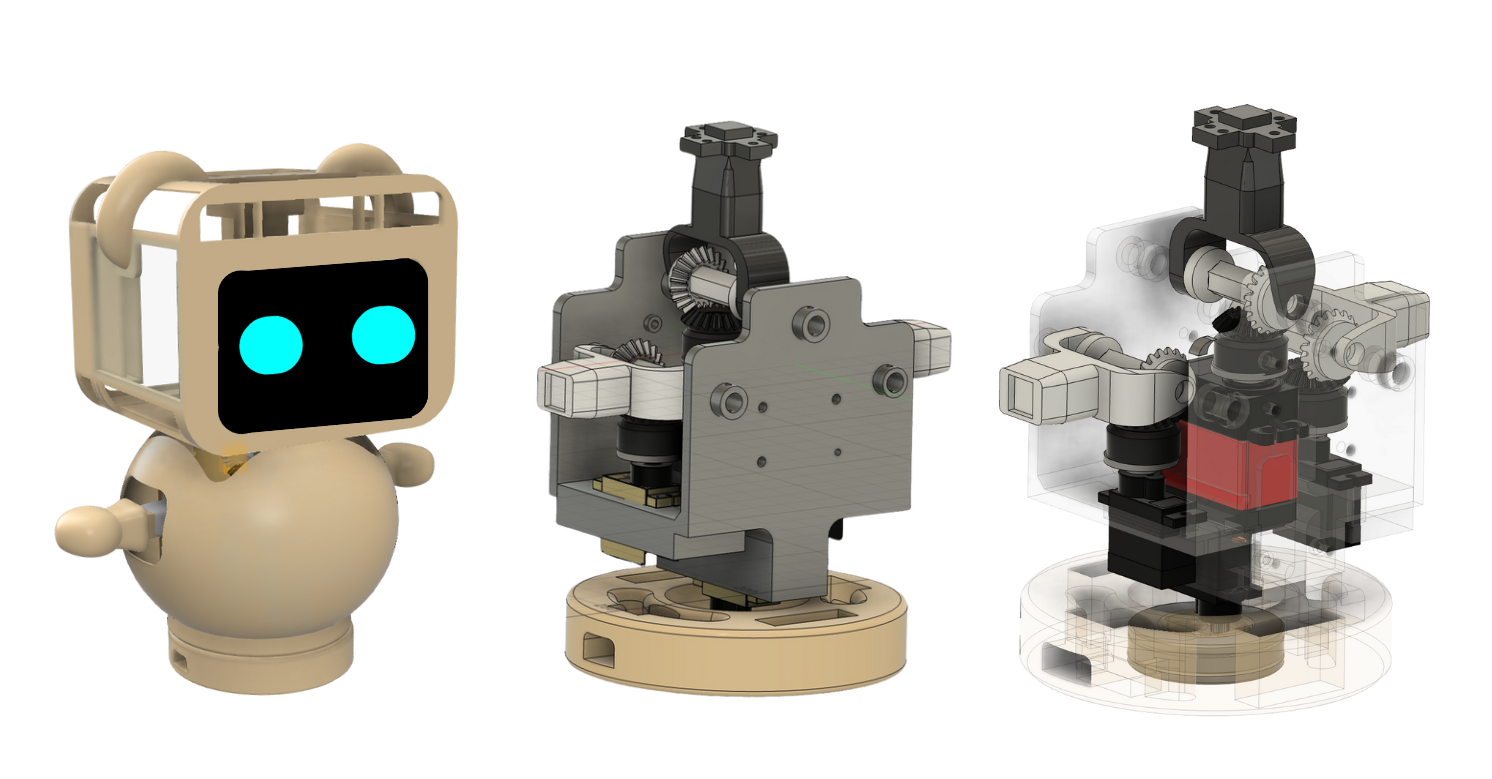
\includegraphics[width=\textwidth]{16-interior.png}
    \captionsetup{justification=centering}
    \caption{Interior Components of Pookie}
    \label{fig:16-interior}
\end{figure}

To enhance design efficiency and modularity, all motors are strategically positioned on a common plane, driving rotational motion along the z-axis. This layout not only simplifies the mechanical structure but also facilitates easier maintenance and part replacement. As shown in Figure \ref{fig:17-kinematics}, a bevel gear system is employed to transfer motion across axes, allowing Pookie to perform complex movements despite having its actuators located in a single plane. This approach optimizes space usage while maintaining full functionality across multiple degrees of freedom. 

\begin{figure}[!ht]
    \centering
    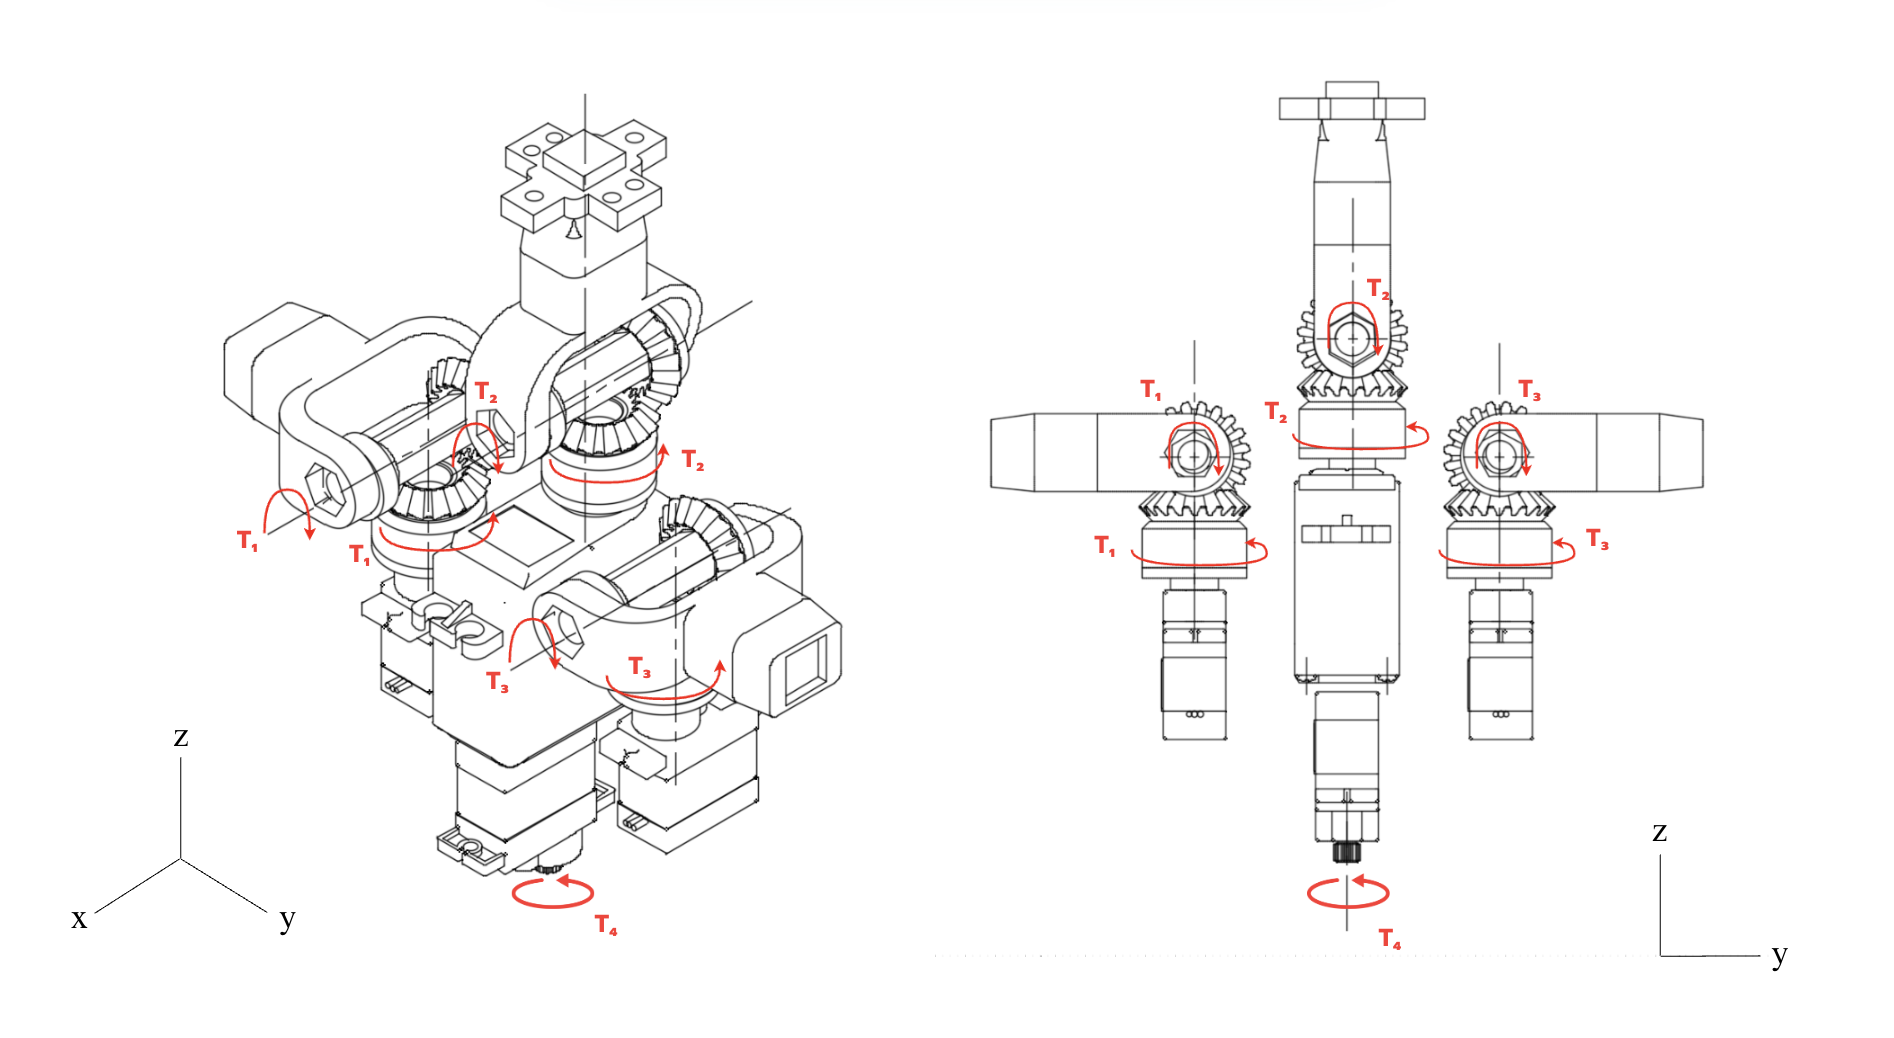
\includegraphics[width=\textwidth]{17-kinematics.png}
    \captionsetup{justification=centering}
    \caption{Pookie Kinematics}
    \label{fig:17-kinematics}
\end{figure}

The bevel gear system is all equal in the number of gear teeth (n). Thus, according to the governing equation for gear ratios shown below, an equal amount of gear teeth constitutes a 1:1 transmission in torque (T). This rule holds true if Pookie comprises a rigid body. 

\begin{gather}
    \frac{n_1}{n_2} = \frac{T_2}{T_1}
\end{gather}

Given this design, two mechanical concerns arise: the torque required to move the head and the load on the base. For torque, Pookie’s arms are lightweight, composed only of a hollow 3D-printed hand and a few embedded magnets. This minimal mass requires very little torque, making the MG90S motor—with a torque rating of 0.18 to 0.22 N·m—an appropriate choice.

In contrast, Pookie’s head contains multiple heavier components, including the LCD screen, wiring adapters, and structural elements, which place a significantly greater torque demand on the motor. While the arms may require less than 0.2 N·m of torque to operate, the head demands over 0.8773 N·m just to remain stable under static conditions. To accommodate this, the TD-8125MG digital servo was selected, delivering a holding torque of 2.31 to 2.63 N·m, which provides a robust safety margin at approximately three times the necessary torque.

The second concern is the vertical load placed on the base motor, responsible for rotating the robot along the z-axis. This motor supports a vertical load exceeding 10 N, resulting from the combined weight of the robot’s upper body and mechanical components. Relying solely on the motor shaft for this axial load would risk rapid wear or mechanical failure. To address this, thrust ball bearings were integrated into the base assembly. Specifically, the team leveraged a 51105 Single direction thrust ball bearing, as there is no radial load on the base.

\begin{figure}[!ht]
    \centering
    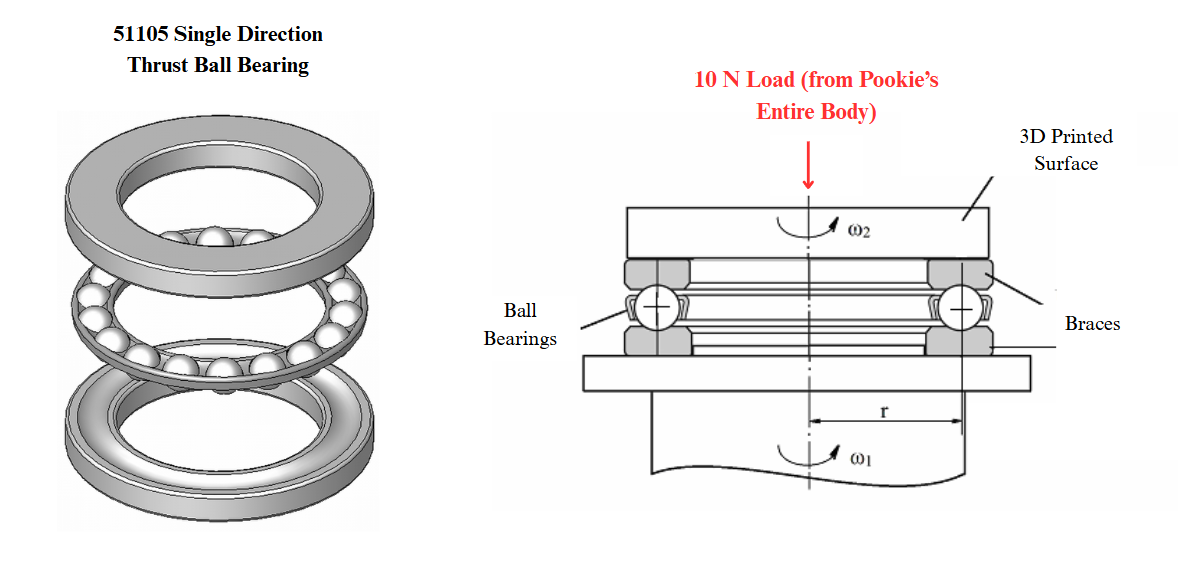
\includegraphics[width=\textwidth]{18-bearings.png}
    \captionsetup{justification=centering}
    \caption{Thrust Ball Bearing. Source: Adapted from \cite{Olaru_2016}}
    \label{fig:18-bearings}
\end{figure}

These specialized bearings are designed to handle high axial loads efficiently, transferring vertical forces away from the motor shaft and distributing them across a broader surface. This ensures smoother rotation, reduces friction, and significantly extends the motor’s operational lifespan.

